\documentclass[12pt, a4paper]{article}
% --- 基础宏包 ---
\usepackage[UTF8]{ctex}     % 中文支持
\usepackage{geometry}       % 页面布局
\usepackage{hyperref}       % 超链接支持
\usepackage{natbib}
\usepackage{booktabs}
\usepackage{newtxtext}      
\usepackage{newtxmath}      
\usepackage{multicol}
\usepackage{multirow}
\usepackage{bm}
\usepackage{natbib}
\let\Bbbk\relax
\usepackage{amssymb}

\usepackage{algorithm}
%\usepackage{algorithmic}
\usepackage{algpseudocode}
\usepackage{graphicx}
\usepackage{subfig}
\usepackage{float}
\usepackage{amsmath}
% --- 页面设置 ---
\geometry{left=1in, right=1in, top=1in, bottom=1in}

% --- 标题信息 ---
\title{\textbf{网约车个体补贴分配仿真研究方案}}

\begin{document}
% 标量用默认字体
% 向量用 \bm
% 集合用大写字母
% 向量集合用 \mathcal
%\citeauthor
\maketitle


\section{研究背景与问题陈述}
在网约车平台的运营决策中，个体补贴分配是调节供需平衡、提升用户留存及最大化平台总交易额的核心方式。

% 带作者姓名引用：\textcite{条目名} → 效果：Chen et al. (2023)
根据现有研究，该问题被数学建模为多选择背包问题（Multiple-Choice Knapsack Problem, MCKP）。其核心在于：针对每一个出行请求（Request/Bubble，$i$），从有限的补贴策略集合（Treatments，$j \in J$）中选择一个最优动作$z_{ij}$，使得总收益$\sum_i\sum_j v_{ij}z_{ij}$最大化，同时满足总预算约束。

\begin{equation} \label{eq:mckp}
\begin{aligned}
\max_{\bm{z}} \quad & \sum_{i} \sum_{j} v_{ijk} z_{ij} \\
\text{s.t.} \quad & \sum_{i}\sum_{j} c_{ij} z_{ij} \le B  \\
& \sum_{j} z_{ij} = 1, \quad \forall i \\
& z_{ij} \in \{0, 1\}, \quad\forall i,\forall j
\end{aligned}
\end{equation}
\begin{itemize}
    \item $i$：表示每一条定价样本，即冒泡
    \item $j \in J$：表示待选的折扣
    \item $v_{ij}$：表示冒泡$i$在折扣 $j$下的收益
    \item $c_{ij}$：表示冒泡$i$在折扣 $j$下的补贴金额
    \item $z_{ij}$：决定对于冒泡$i$是否选择折扣$j$的决策变量
    \item $B$：表示总补贴额
\end{itemize}

目前主流解法采用拉格朗日松弛（Lagrangian Relaxation）引入拉格朗日乘子,将全局约束问题转化为个体的无约束问题：
$$j^*=\max_j (v_{ij} - \lambda c_{ij})$$
$$z_{ij} = 
\begin{cases} 
1 & \text{if } j = j^*\\ 
0& \text{otherwise} 
\end{cases}$$

在理想的静态环境下，该方法能通过获得近似最优解。然而，在实际的动态环境与在线决策环节中，$\lambda$的求解面临两大挑战，制约了策略的有效性：

1、离线-在线分布偏差：

仿真求解的是“离线数据分布”下的最优解，假设是离线数据和在线数据分布一致，并且为了尽可能满足这个假设，会使用最近的一周历史数据分布近似替代线上的数据分布。然而在线上应用时，数据分布发生改变，不同分布下的全局最优解是不同的。
例如在依据2026年1月8号-1月14号的历史数据去近似2026年2月2号-2月8号的数据。统计仿真数据和线上数据分天的数据分布情况，两者如下：

\begin{figure}[!h]
    \centering
    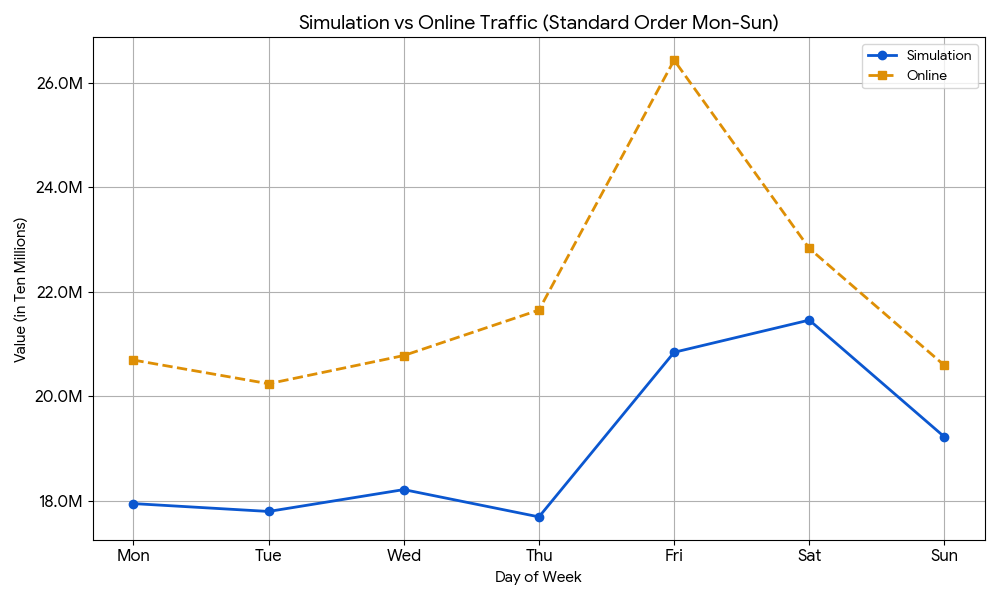
\includegraphics[width=5in]{figures/仿真与线上分布.png}
    \caption{仿真与实际偏移数据}
    \label{fig:my_label}
\end{figure}

因此，如何在未来在线数据未知的情况下，更好地用历史数据近似替代未来现实的数据分布，是解决仿真偏差的核心。

2、$\lambda$为固定值的局限性：

当前仿真产出的$\lambda$是一个全局固定的标量值。这意味着系统假设单位预算的边际价值对于所有用户、所有时空场景都是是均等的。然而，实际业务中存在显著的异质性、不确定性。因此仿真产出的应该是一个“补贴率-> $\lambda$分布”的字典。

\section{研究目标与方案概述}

针对上述两个挑战，提出两个仿真的改进方向：

1、离线与在线数据分布对齐的偏差矫正模块：
通过引入密度比估计（Density Ratio Estimation）等方法，对离线仿真数据进行重加权或特征对齐，使得离线数据的分布特性最大程度贴合在线真实分布，从而直接修正仿真评估的系统性偏差。

2、基于特征与补贴率的$\lambda$分布预测模型：
将$\lambda$的求解从“仿真遍历搜索出的单一固定值”升级为“由深度学习模型预测出的条件概率分布”。该模型以上下文特征（相比线上有一小时延迟的准实时数据）和目标补贴率为输入，产出$\lambda$的概率分布。最终，仿真过程将产出一个“补贴率 -> $\lambda$分布”的字典表，不同的补贴率将映射到不同的$\lambda$分布上。在线决策时，系统查表获取对应补贴率下的$\lambda$分布，从而实现动态的$\lambda$调节。

\section{研究指标与具体方案}
\begin{figure}[!h]
    \centering
    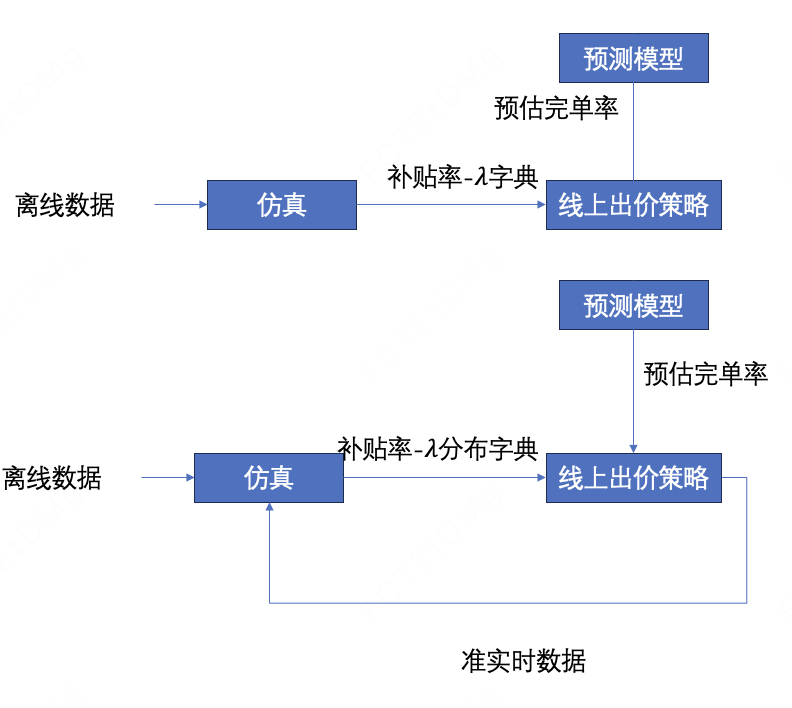
\includegraphics[width=5in]{figures/仿真研究方案.png}
    \caption{仿真研究方案}
    \label{fig:my_label}
\end{figure}

\subsection{研究方案模块一}基于准实时数据的“分布-规模”双重校准模块
\subsubsection{问题分析}分类器校准的局限性与规模偏差

仿真失真的核心在于“离线数据”无法代表“在线环境”，这体现在两个维度：分布形状（Shape）偏移;绝对规模（Volume）偏差。

传统分类器的缺陷：如果我们仅训练一个分类器 $D(x)$ 来区分样本来自“离线”还是“在线”，并计算密度比 $w(x) = \frac{P_{on}(x)}{P_{off}(x)}$，这个权重本质上是在概率密度空间进行操作的。它会把离线数据的分布“拉扯”成在线数据的形状，但加权后的样本总权重之和，依然等于离线样本的数量，而不是在线数量。对于涉及绝对金额预算 $B$ 的优化问题，这种规模丢失（Volume Loss）会导致仿真低估总消耗，从而计算出错误的 $\lambda$（偏低），上线后引发预算超支。

\subsubsection{改进方法}双重校准机制（Dual-Calibration Mechanism）

我们提出利用可获取的准实时数据（现实世界1小时前的数据），构建一个包含形状校准和规模校准的双层纠偏模块。

第一层：基于分类器的形状校准（Shape Calibration）利用密度比估计（Density Ratio Estimation）解决特征分布（相对比例）不一致的问题。数据准备：$D_{off}$：离线历史数据（有标签，量级较小或不全）。$D_{real}$：准实时在线数据（无标签，仅有特征 $X$，代表最新的真实分布）。模型训练：训练一个二分类器（如LightGBM），区分样本来自 $D_{off}$ (Label=0) 还是 $D_{real}$ (Label=1)。形状权重计算：$$w_{shape}(x) = \frac{P(real|x)}{P(off|x)} \cdot \frac{N_{off}}{N_{real}}$$（注：乘上先验比例 $\frac{N_{off}}{N_{real}}$ 是为了消去分类器训练时的样本不平衡影响，还原纯粹的密度比 $\frac{p_{real}(x)}{p_{off}(x)}$）。

第二层：基于流量统计的规模校准（Volume Calibration。利用准实时数据流的统计信息，实时统计当前在线环境的单位时间请求量，记为 $V_{real}$。离线流量统计：统计离线仿真数据集中对应时间段的请求量，记为 $V_{off}$。规模权重计算：$$w_{scale} = \frac{V_{real}}{V_{off}}$$

逻辑链路与预期效果逻辑链路：

利用滞后一小时的准实时数据，针对特征分布的非平稳变化（如突发天气导致的高价值用户激增）以及流量统计的偏差，通过实时调优样本权重 $w_{shape}$ 来修正分类器偏差，最大化模型在当前环境下的泛化能力。


\subsection{研究方案模块二}产出“补贴率 -> Lambda分布”字典的预测模型

\subsubsection{问题分析}

静态标量字典的局限性与多解空间在既有仿真中，产出物通常是一个将目标补贴率映射为固定标量 $\lambda$ 的字典表。此范式在理论上存在显著缺陷：
多解空间的坍缩：在期望补贴率（SR）的非线性约束下，映射关系失去了单调双射性质，同一个补贴率实际上对应一个候选的 $\lambda$ 集合。
忽略异质性不确定性：影子价格 $\lambda$ 表征单位预算的边际价值。由于环境的高度时变性和个体特征的差异，固定的 $\lambda$ 无法响应系统动态。$\lambda$ 在本质上应当是一个以当前时序上下文特征与目标约束为条件的概率分布。更为关键的是，由于资源稀缺度的不同，不同的补贴率约束必然诱导出形态截然不同的Lambda分布。

\subsubsection{改进方法}构建条件Lambda分布预测与字典表映射模型

提出构建一个深度概率生成模型 $M_\Lambda$，将拉格朗日乘子的求解升级为分布预测任务。

模型的条件特征输入模型 $M_\Lambda$ 旨在拟合多解空间下的条件概率密度函数，其输入空间需充分捕捉系统的时间动态：空间与状态特征（$X_t$）：当前请求的用户属性、微观供需状态。近期时序状态表征（Recent Temporal State Representations, $X_{t-\Delta t}$）：引入系统近期的宏观统计特征（如近1小时的全局应答率、预算消耗速率），利用时序网络提取时序演进模式，使模型具备对环境漂移的自适应感知能力。目标补贴率约束（$SR$）：作为条件生成的核心控制变量。

仿真产出：参数化分布字典的构建在经过双重校准后的仿真遍历流程中：
针对每一个给定的目标补贴率 $SR$，结合数据集中丰富的上下文与时序状态组合 $(X_t, X_{t-\Delta t})$，模型 $M_\Lambda$ 拟合出该约束条件下全局 $\lambda$ 的概率分布规律 $P(\lambda |SR)$。

字典结构的重构：仿真最终的输出实体将从标量映射升级为分布参数映射字典表：（分布参数可为均值 $\mu$、方差 $\sigma^2$、偏度或非参数化的分位数向量）。




\end{document}